

\begin{frame}
    \frametitle{Sleep modes}
    With sleep modes, it is possible to reduce the energy consumption by disabling modules that are not used.
    The ESP8266 provides three different sleep modes:
    \begin{itemize}
        \item Modem sleep (default)
        \item Light sleep
        \item Deep sleep
    \end{itemize}
\end{frame}

\begin{frame}
    \frametitle{Sleep modes}
    \framesubtitle{Current consumption / Datasheet}

    \begin{table}[htbp]
        \caption{ESP8266 sleep modes}
        \begin{center}
        \begin{tabular}{|c|c|c|c|}
        \hline
        \textbf{Module}&\textbf{Modem sleep}&\textbf{Light sleep}&\textbf{Deep sleep}\\
        \hline
        \textbf{WiFi} & OFF & OFF & OFF\\
        \textbf{AP association} & Connected & Connected & Disconnected\\
        \textbf{System clock} & ON & OFF & OFF\\
        \textbf{RTC} & ON & ON & ON\\
        \textbf{CPU} & ON & Pending & OFF\\
        \hline
        \textbf{Substrate current} & $15mA$ & $0.4mA$ & $20\mu A$\\
        \hline
        \end{tabular}
        \label{tab_sleep_modes}
        \end{center}
    \end{table}
\end{frame}

\begin{frame}
    \frametitle{Sleep modes}
    \framesubtitle{Modem sleep / Light sleep}

    \begin{minipage}{0.45 \textwidth}
        \begin{figure}[H]
            \centering
            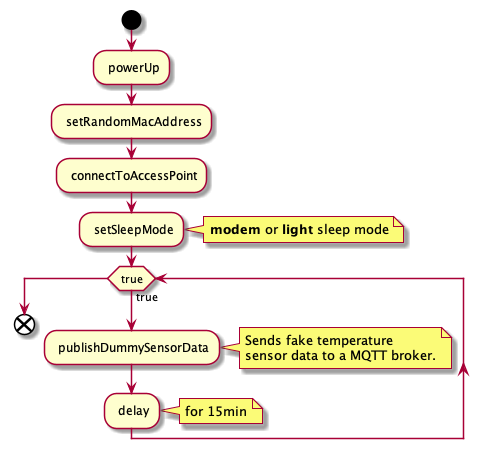
\includegraphics[width = 1 \linewidth]{../paper/fig/sequence_modem_light_sleep.png}
            \caption{Experimental setup for modem and light sleep.}
            \label{fig:experiment_modem_light_sleep}
        \end{figure}
    \end{minipage}
    \begin{minipage}{0.45 \textwidth}
        \begin{itemize}
            \item Experimental setup Modem- and Light- sleep.
            \item ESP8266 stays connected to the AP
        \end{itemize}
    \end{minipage}
\end{frame}


\begin{frame}
    \frametitle{Sleep modes}
    \framesubtitle{Modem sleep Results}

    \begin{minipage}{0.45 \textwidth}
        \begin{figure}[H]
            \centering
            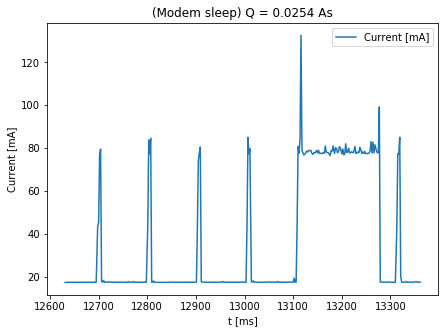
\includegraphics[width = 1 \linewidth]{../paper/fig/modem_sleep.png}
            \caption{Current trace modem sleep}
            \label{fig:experiment_modem_light_sleep}
        \end{figure}
    \end{minipage}
    \begin{minipage}{0.45 \textwidth}
        \begin{itemize}
            \item $I_{idle} \approx 18mA$
            \item $I_{transmission} \approx 80mA$
            \item Beacons processed every $100m$
        \end{itemize}
    \end{minipage}
\end{frame}

\begin{frame}
    \frametitle{Sleep modes}
    \framesubtitle{Light sleep Results}

    \begin{minipage}{0.45 \textwidth}
        \begin{figure}[H]
            \centering
            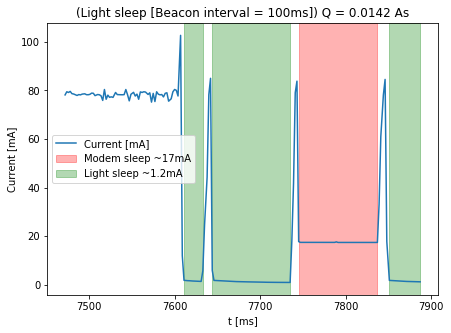
\includegraphics[width = 1 \linewidth]{../paper/fig/light_sleep.png}
            \caption{Current trace light sleep}
            \label{fig:experiment_modem_light_sleep}
        \end{figure}
    \end{minipage}
    \begin{minipage}{0.45 \textwidth}
        \begin{itemize}
            \item $I_{idle_{modem}} \approx 17mA$
            \item $I_{idle_{light}} \approx 1.2mA$
            \item $I_{transmission} \approx 80mA$
            \item Beacons also processed every $100ms$
            \item Controller switches automatically between \textbf{modem} and \textbf{light} sleep.
        \end{itemize}
    \end{minipage}
\end{frame}


\begin{frame}
    \frametitle{Sleep modes}
    \framesubtitle{Deep sleep}

    \begin{minipage}{0.45 \textwidth}
        \begin{figure}[H]
            \centering
            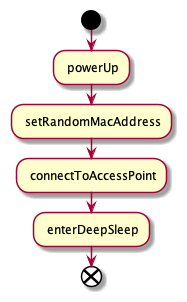
\includegraphics[width = 1 \linewidth]{../paper/fig/sequence_deep_sleep.png}
            \caption{Experimental setup for deep sleep.}
            \label{fig:experiment_modem_light_sleep}
        \end{figure}
    \end{minipage}
    \begin{minipage}{0.45 \textwidth}
        \begin{itemize}
            \item Experimental setup deep sleep.
            \item ESP8266 is \textbf{disconnected} from the AP.
        \end{itemize}
    \end{minipage}
\end{frame}

\begin{frame}
    \frametitle{Sleep modes}
    \framesubtitle{Deep sleep Results}

    \begin{minipage}{0.45 \textwidth}
        \begin{figure}[H]
            \centering
            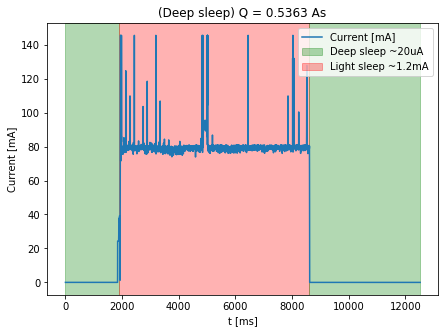
\includegraphics[width = 1 \linewidth]{../paper/fig/deep_sleep.png}
            \caption{Current trace deep sleep}
            \label{fig:experiment_modem_light_sleep}
        \end{figure}
    \end{minipage}
    \begin{minipage}{0.45 \textwidth}
        \begin{itemize}
            \item $I_{idle} \approx 20 \mu A$
            \item $I_{transmission} \approx 80mA$
            \item Controller is \textbf{disconnected} from the AP.
        \end{itemize}
    \end{minipage}
\end{frame}


\begin{frame}
    \frametitle{Sleep modes}
    \framesubtitle{Comparison}

    \begin{itemize}
        \item We measured the used energy in $[As]$ over $10$ cycles, with a sleep interval of $15min$.
    \end{itemize}

    \begin{table}[htbp]
        \caption{Measured sleep power consumption}
        \begin{center}
        \begin{tabular}{|c|c|c|}
        \hline
        \textbf{Sleep mode}&\textbf{Used energy $[As]$}&\textbf{Average current $[mA]$}\\
        \hline
        \textbf{Modem sleep} & 323.77As & 36.9mA\\
        \textbf{Light sleep} & 182.31As & 20.46mA\\
        \textbf{Deep sleep}  & 1.12As   & 0.127mA\\
        \hline
        \end{tabular}
        \label{tab:sleep_modes_15min}
        \end{center}
    \end{table}

    \pause

    \begin{tcolorbox}[title=Energy saving, colback=blue!10, colframe=blue!40]
        We were able to \textbf{reduce the energy consumption} by a factor of \textbf{$\approx 290$}, compared to the default modem sleep mode.
    \end{tcolorbox}
    
\end{frame}